\documentclass[12pt]{report}
\usepackage[utf8]{inputenc}
\usepackage[russian]{babel}
\usepackage{setspace} % для междустрочного интервала
\onehalfspacing % 1.5 интервал между строками

\usepackage[left=30mm, top=20mm, right=20mm, bottom=20mm, nohead, footskip=7mm]{geometry}

\usepackage{titlesec, blindtext, color} 
\definecolor{gray75}{gray}{0.75}
\newcommand{\hsp}{\hspace{20pt}}
\titleformat{\chapter}[hang]{\Large\bfseries}{\thechapter{. }}{0pt}{\Large\bfseries}
\titlespacing{\chapter}{-5pt}{-30pt}{12pt} % отступ заголовка сверху
\titleformat{\section}[hang]{\large\bfseries}{\thesection{. }}{0pt}{\large\bfseries}

\makeatletter % список литературы
\def\@biblabel#1{#1. }
\makeatother

% Ссылки
\usepackage{hyperref}

% Возможность вставки pdf страниц
\usepackage{pdfpages}

% Листинги
\usepackage{listings}

% Для возможности переноса строк в equation, только надо еще и окружение \begin{gathered} сделать
\usepackage{amsmath}

\lstset{
	language = c++,
	extendedchars=\true,
	basicstyle=\small\sffamily,
	numbers=left,
	numberstyle=\tiny,
	stepnumber=1,
	numbersep=5pt,
	showspaces=false,            % показывать или нет пробелы специальными отступами
	showstringspaces=false,
	showtabs=false,
	frame=single,
	tabsize=2,
	captionpos=t,
	breaklines=true,
	breakatwhitespace=false,
	escapeinside={\#*}{*)},
	keepspaces=true
}

% Чтобы вместо : в подписях было -
\RequirePackage{caption}
\DeclareCaptionLabelSeparator{defffis}{ — }
\captionsetup{justification=centering,labelsep=defffis}

\usepackage{pgfplots}
\usepackage{pgfplotstable}
\pgfplotsset{compat=1.9}


\usepackage{csvsimple} %
\usepackage{datatool}




\begin{document}
	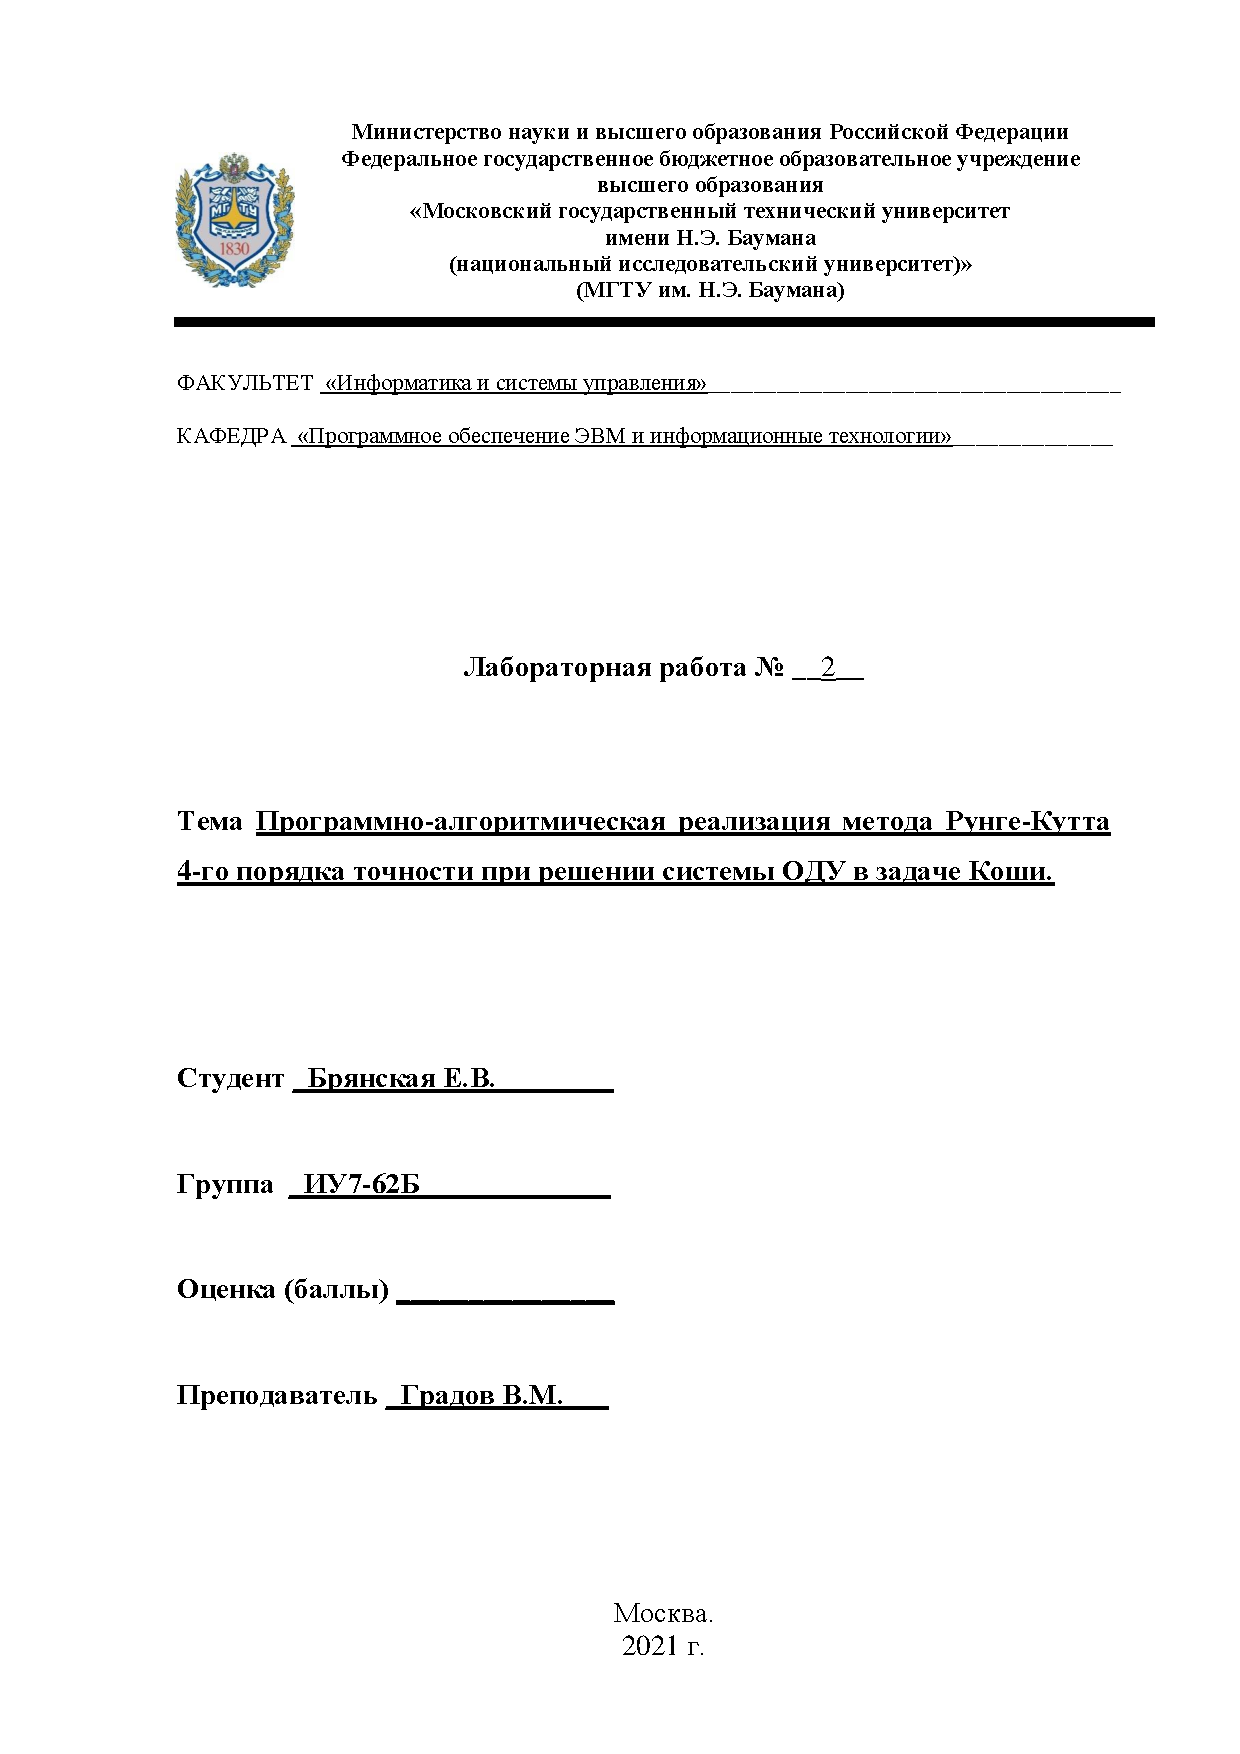
\includepdf[pages=1]{title.pdf}
	
	\chapter*{Задание}

\textbf{Тема. } Программно- алгоритмическая реализация моделей на основе ОДУ второго порядка
с краевыми условиями II и III рода.\\

\textbf{Цель работы. } Получение навыков разработки алгоритмов решения краевой задачи при
реализации моделей, построенных на ОДУ второго порядка. \\

\textbf{Исходные данные. }\\
\begin{enumerate}
	\item Задана математическая модель. \\
	Квазилинейное уравнение для функции T(x)
	
	\begin{equation}\label{formula1}
		\frac{d}{dx}\bigg(\lambda(T)\frac{dT}{dx}\bigg) - 4 \cdot k(T) \cdot n_p^{2} \cdot \sigma \cdot (T^4 - T_0^4) = 0
	\end{equation}

	Краевые условия:
	\begin{equation}\label{formula2}
		\left\{
		\begin{array}{ccc}
			x = 0, -\lambda(T(0))\frac{dT}{dx} = F_0,\\
			x = l, -\lambda(T(l))\frac{dT}{dx} = \lambda(T(l) - T_0) \\
		\end{array}
		\right.
	\end{equation}

	\item Функции $\lambda(T), k(T)$ заданы таблицей
	\begin{table}[ph!]\label{table_1}
		\caption{}
		\centering
		\begin{tabular}{|c|c|c|c|c|}
			\hline
			$T, K$ & $\lambda$, Вт/(см К) & & $T, K$ & $k,$ см(-1)\\
			\hline
			300 & $1.36 \cdot 10^{-2}$ && 293 & $2.0 \cdot 10^{-2}$\\
			\hline
			500 & $1.63 \cdot 10^{-2}$ && 1278 & $5.0 \cdot 10^{-2}$\\
			\hline
			800 & $1.81 \cdot 10^{-2}$ && 1528 & $7.8 \cdot 10^{-2}$ \\
			\hline
			1100 & $1.98 \cdot 10^{-2}$ && 1677 & $1.0 \cdot 10^{-1}$ \\
			\hline
			2000 & $2.50 \cdot 10^{-2}$ && 2000 & $1.3 \cdot 10^{-1}$ \\
			\hline
			2400 & $2.74 \cdot 10^{-2}$ && 2400 & $2.0 \cdot 10^{-1}$ \\
			\hline
	
		\end{tabular}
	\end{table}

	\item Разностная схема с разностным краевым условием при $x = 0$. Получена в Лекции №7, и может быть использована в данной работе. Самостоятельно надо получить интегро-интерполяционным методом разностный аналог краевого условия при $x = l$, точно
	так же, как это было сделано применительно к краевому условию при $x = 0$ в указанной 
	лекции. Для этого надо проинтегрировать на отрезке $[x_{N-\frac{1}{2}}, x_N]$ записанное выше уравнение \ref{formula1} и учесть, что поток $F_N = \alpha_N(y_N - T_0)$, а $F_{N - \frac{1}{2}} = \chi_{N - \frac{1}{2}}(\frac{y_{N-1} - y_N}{h})$
	
	\item Значения параметров для отладки (все размерности согласованы)
	$n_p$ = 1.4 – коэффициент преломления,
	l = 0.2 см – толщина слоя,
	$T_0$ = 300К – температура окружающей среды,
	$\sigma$ = $5.668 \cdot 10_{-12}$ Вт/(см2K4) - постоянная Стефана- Больцмана,
	$F_0$ = 100 Вт/см2 - поток тепла,
	$\alpha$ = 0.05 Вт/(см2 К) – коэффициент теплоотдачи. 
	
	\item  Выход из итераций организовать по температуре и по балансу энергии, т.е.
	\begin{equation}\label{formula3}
		max \bigg|\frac{y_n^s - y_n^{s-1}}{y_n^s} \bigg| \leq \varepsilon_1, n = 0, 1, ..., N
	\end{equation}

	\begin{equation}\label{formula4}
		max \bigg|\frac{f_1^s - y_2^s}{f_1^s} \bigg| \leq \varepsilon_2
	\end{equation}
	
	где 
	\begin{equation}\label{formula5}
		f_1 = F_0 - \alpha(T(l) - T_0)
	\end{equation}
	и
	\begin{equation}\label{formula6}
		f_2 = 4n_p^2 \sigma \int_0^l k(T(x))(T^4(x) - T_0^4)dx
	\end{equation}
	
\end{enumerate}






	\chapter*{Выполнение}

Задача решается методом Рунге-Кутта 4ого порядка для системы ОДУ.\\
\begin{equation}
	y_{n + 1} = y_n + \frac{k_1 + 2k_2 + 2k_3 + k_4}{6},
	~~~~~~~~z_{n + 1} = z_n + \frac{p_1 + 2p_2 + 2p_3 + p_4}{6}
\end{equation}

где

\begin{equation}
	k_1 = hf(x_n, y_n, z_n)    
	~~~~~~~~p_1 = h\varphi(x_n, y_n, z_n)
\end{equation}

\begin{equation}
	k_2 = hf(x_n + \frac{h}{2}, y_n + \frac{k_1}{2}, z_n + \frac{p_1}{2})    
	~~~~~~~~p_2 = h\varphi(x_n + \frac{h}{2}, y_n + \frac{k_1}{2}, z_n + \frac{p_1}{2})
\end{equation}

\begin{equation}
	k_3 = hf(x_n + \frac{h}{2}, y_n + \frac{k_2}{2}, z_n + \frac{p_2}{2})    
	~~~~~~~~p_3 = h\varphi(x_n + \frac{h}{2}, y_n + \frac{k_2}{2}, z_n + \frac{p_2}{2})
\end{equation}

\begin{equation}
	k_4 = hf(x_n + \frac{h}{2}, y_n + k_3, z_n + p_3)    
	~~~~~~~~p_4 = h\varphi(x_n + \frac{h}{2}, y_n + k_3, z_n + p_3)
\end{equation}



	\section*{Результат работы программы.}
\begin{enumerate}
	\item Графики зависимости от времени импульса $t$: $I(t), U(t), R_p(t),$ произведения $I(t) \cdot R_p(t), T_0(t)$ при заданных выше параметрах.
	Шаг сетки - $10^{-7}$.
	
	\begin{figure}[h]
		\begin{center}
			{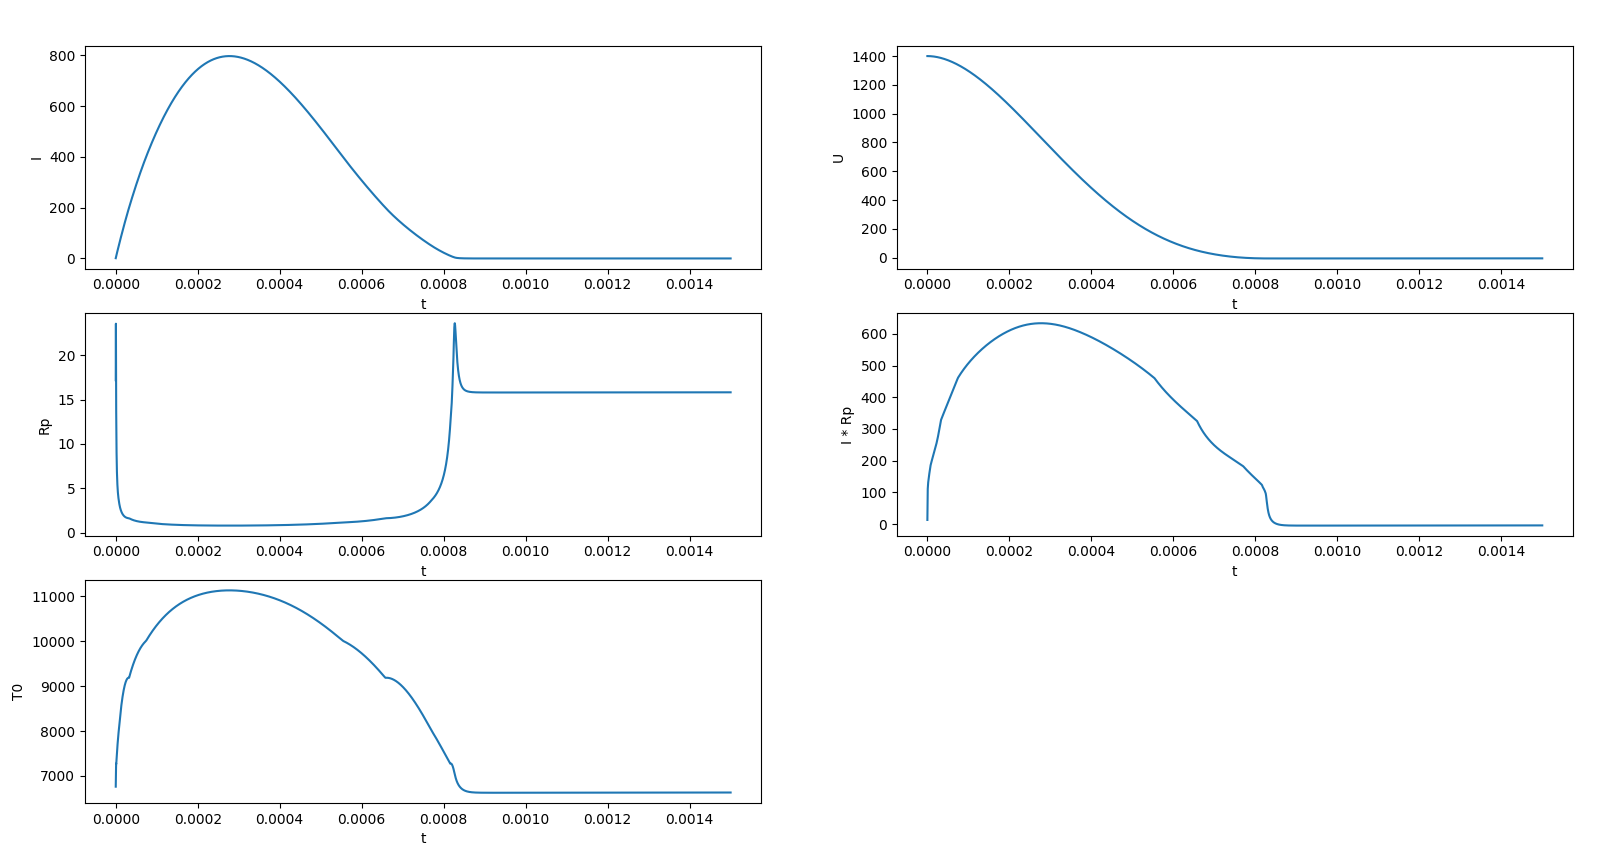
\includegraphics[height=9.5cm, width = 18cm]{tasks/task_1}}
		\end{center}
	\end{figure}
	
	\item График зависимости $I(t)$ при $R_k + R_p = 0$. Обратить внимание на то, что в этом случае колебания тока будут незатухающими.
	
	\begin{figure}[h]
		\begin{center}
			{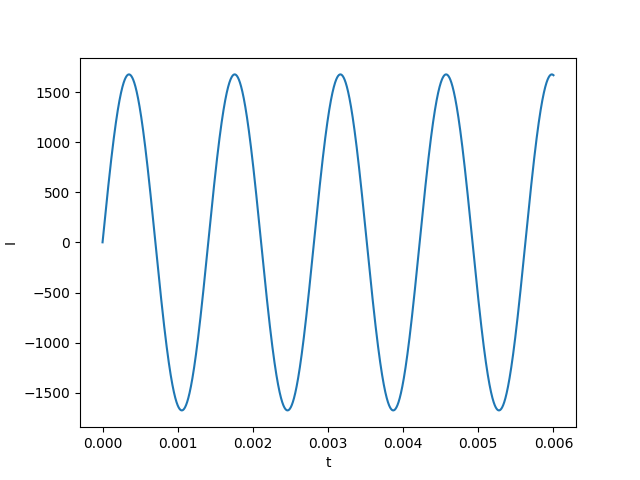
\includegraphics[height=9cm, width = 16cm]{tasks/task_2}}
		\end{center}
	\end{figure}
	
	\item График зависимости $I(t)$ при $R_k + R_p = const = 200$ Ом в интервале значений $t$ 0-20 мкс.
	
	\begin{figure}[h]
		\begin{center}
			{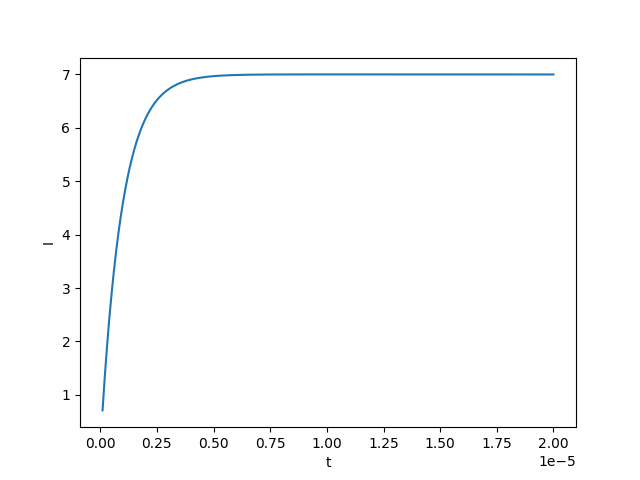
\includegraphics[height=7.76cm, width = 16cm]{tasks/task_3}}
		\end{center}
	\end{figure}
	
	\item Результаты исследования влияния параметров контура $C_k, L_k, R_k$ на длительность импульса tимп. апериодической формы. Длительность импульса определяется по кривой зависимости тока от времени на высоте
	$35 I_{max}, I_{max}$ - значение тока в максимуме (см. рисунок).
	
	\begin{figure}[h]
		\begin{center}
			{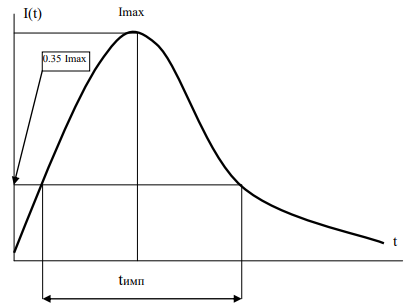
\includegraphics[height=3.3cm, width =8cm]{graph}}
		\end{center}
	\end{figure}
	
	\begin{table}[ph!]\label{table_3}
		\caption{Влияние $C_k$ на длительность импульса tимп}
		\centering
		\begin{tabular}{|c|c|c|c|c|c|c|c|c|c|c|}
			\hline
			$C_k$, мкФ & 200 & 250 & 300 & 350 & 400 & 450 & 500 & 550 & 600 & 650\\
			\hline
			tимп, мкс & 485.10 & 546.10 & 602.10 & 654.20 & 703.20 & 749.90 & 794.70 & 838.0 & 879.70 & 920.40\\
			\hline	
		\end{tabular}
	\end{table}
	
	\begin{table}[ph!]\label{table_4}
		\caption{Влияние $L_k$ на длительность импульса tимп}
		\centering
		\begin{tabular}{|c|c|c|c|c|c|c|c|c|c|c|}
			\hline
			$L_k$, мкГн & 100 & 150 & 200 & 250 & 300 & 350 & 400 & 450 & 500 & 550 \\
			\hline
			tимп, мкс & 425.50 & 511.80 & 584.70 & 649.30 & 708.20 & 762.50 & 813.20 & 861.00 & 906.20 & 949.20\\
			\hline	
		\end{tabular}
	\end{table}
	
	\begin{table}[ph!]\label{table_5}
		\caption{Влияние $R_k$ на длительность импульса tимп}
		\centering
		\begin{tabular}{|c|c|c|c|c|c|c|c|c|c|c|c|}
			\hline
			$R_k$, Ом & 0.1 & 0.2 & 0.4 & 0.6 & 0.8 & 1.0 & 1.2 & 1.4 & 1.6 & 1.8 & 2.0 \\
			\hline
			tимп, мкс & 556.20 & 562.90 & 580.2 & 604.5 & 636.3 & 675.3 & 723.9 & 781.01 & 842.6 & 903.2 & 959.7\\
			\hline	
		\end{tabular}
	\end{table}
	
	\begin{figure}[ph!]
		\begin{center}
			{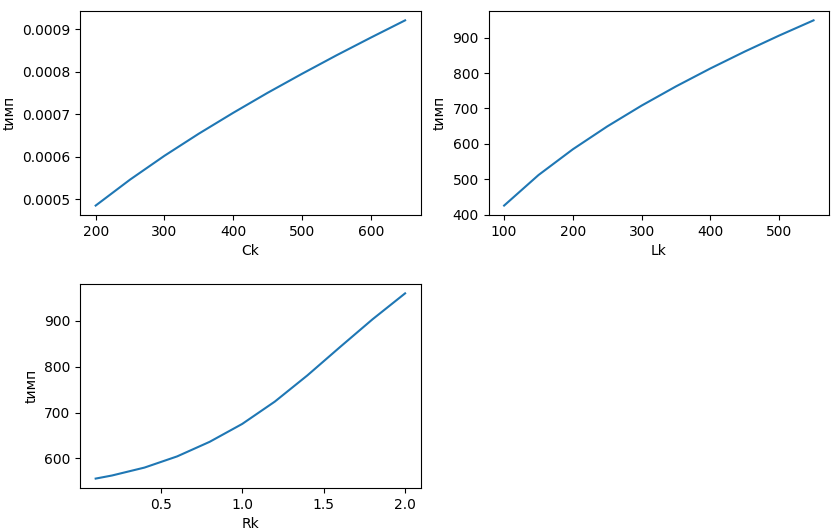
\includegraphics[height=7.58cm, width = 16cm]{tasks/task_4}}
		\end{center}
	\end{figure}
	В результате исследования было выявлено, что при увеличении любого из трёх параметров увеличивается и длительность импульса.
	
\end{enumerate}
	\underline{\textbf{Вопросы при защите лабораторной работы}}\\

\begin{enumerate}
\item \textbf{Укажите интервалы значений аргумента, в которых можно считать решением заданного уравнения каждое из первых 4-х приближений Пикара. Точность результата оценивать до второй цифры после запятой. Объяснить свой ответ.}

\item \textbf{Пояснить, каким образом можно доказать правильность полученного результата при фиксированном значении аргумента в численных методах.}

В силу того, что численные методы зависят от величины шага, то изменяя его, можно прийти к наиболее точному результату при фиксированном значении аргумента. Как только результат перестаёт отличатся от результатов, полученных ранее, то можно сделать вывод о том, что корректный результат получен.

\item \textbf{Каково значение функции при x=2, т.е. привести значение u(2).}

При $x = 2$ и шаге $10^{-6}$ было получено значение функции равное $317.82$.
\end{enumerate}
	\newpage
	\underline{\textbf{Код программы}}

\begin{lstlisting}[label=code1, caption = Лабораторная работа №1]
from math import sqrt

def f(x, y):
	return x**2 + y**2

def picard_1(x_args):
	res = []
	for x in x_args:
		res.append(x**3 / 3)
	return res

def picard_2(x_args):
	res = []
	for x in x_args:
		res.append(x**3 / 3 + x**7 / 63)
	return res

def picard_3(x_args):
	res = []
	for x in x_args:
		res.append(x**3 / 3 + x**7 / 63 + x**15 / 59535 + 2*x**11 / 2079)
	return res

def picard_4(x_args):
	res = []
	for x in x_args:
		res.append(x**3/3 + x**7/63 + x**15/59535 + 2*x**11/2079 +
		x**31/109876902975 + 4*x**23/99411543 + 4*x**27/3341878155 + 2*x**23/86266215 + 2*x**19/3393495 + 4*x**19/2488563 + 4*x**15/93555)
	return res

def runge_kutta(x, y, h, num):
	alpha = 0.5
	res = []
	temp = h / (2 * alpha)
	
	for i in range(num):
		res.append(y)
	
	k1 = f(x, y)
	k2 = f(x + temp, y + temp * k1)
	
	y += h * ((1 - alpha) * k1 + alpha * k2)
	x += h
	
	return res


def euler_explicit(x, y, h, num):
	res = []
	
	for i in range(num):
		res.append(y)
	
	try:
		y += h * f(x, y)
		x += h
	except OverFlowError:
		for k in range(i, num):
			res.append('---')
		break
	return res

def count_x_args(x, x_max, h):
	x_args = []
	while x <= x_max:
		x_args.append(x)
		x += h
	return x_args


def print_head():
	print(' '*4+'x'+' '*4+'|'+' '*17+'Метод Пикара'+' '*18+'|'+' '*6+'Метод Эйлера'+' '*5+'|'+' '*3+'Метод Рунге-Кутта'+' '*3+'\n'+' '*9+'|'+' '*5+'1'+' '*5+'|'+' '*5+'2'+' '*5+'|'+' '*5+'3'+' '*5+'|'+' '*5+'4'+' '*5+'|'+' '*3+'Явный'+' '*3+'\n'+'-'*55)


def main():
	print_head()
	
	x, x_max, y = 0, 2, 0
	h = 10 ** -6
	
	x_args = count_x_args(x, x_max, h)
	
	res_runge_kutta = runge_kutta(x, y, h, num)
	res_euler_explicit = euler_explicit(x, y, h, num)
	res_picard_1 = picard_1(x_args)
	res_picard_2 = picard_2(x_args)
	res_picard_3 = picard_3(x_args)
	res_picard_4 = picard_4(x_args)
	
	for i in range(len(x_args)):
		print('{:9.3f}|{:11.3e}|{:11.3e}|{:11.3e}|{:11.3e}|{:11.3e}|{:11.3e}'.format(x_args[i], res_picard_1[i], res_picard_2[i], res_picard_3[i], res_picard_4[i], res_euler_explicit[i], res_runge_kutta[i]))


if __name__ == '__main__':
	main()
\end{lstlisting}
\end{document}
